\documentclass{beamer}

\usepackage{graphicx}

\title[Earning Classification]
{Classification of Earning from Census Data}
\subtitle{}
\author[Group 25] 
{Miles~Scherrer \and Daniel~Enkvist \and Johannes~Krohn}
\institute[UU]{Uppsala Universitet}
\date[Uppsala October 2016] 
{Data Mining I, 2016}
\subject{Computer Science}

\usetheme{CambridgeUS}
\usecolortheme{dolphin}

\begin{document}
\frame{\titlepage}

\frame{
\frametitle{How the Data Looks Like}	
\begin{itemize}
	\item raw data is a 1\% sample of the original US Census Data from 1990\pause
	\item compressed data....
\end{itemize}
}

\frame{
\frametitle{Preprocessing}	
\begin{itemize} \itemsep1em
	\item removed examples with negative earnings (only a small fraction) \pause
	\item removed income attributes due to high correlation with earnings \pause
	\item romeved all examples with age $< 20$ and age $> 64$ \pause
	\item removed all examples which have n/a values in crucial attributes \pause
	\item split data into training and testing set (90\% for training)
\end{itemize}
	
}

\frame{
\frametitle{Prediction of the 5 Earning Classes}
\framesubtitle{Decision Tree - information\_gain, maximal depth 6, no pruning}
\pause
\begin{itemize}
	\item further preprocessing by \pause
	\begin{itemize}
		\item generating polynomial labels from numerical values \pause
		\item sampling same amount of examples from the five different classes \pause
	\end{itemize}
	\item still too many attributes, so we used the forward selection operator: \pause
	\begin{itemize}
		\item \textbf{dHour89} - usual hours worked per week last year (1989) 
		\item \textbf{iYearsch} - education attainment
		\item \textbf{dWeek89} - weeks worked last year (1989)
		\item \textbf{iFertil} - number of children given birth to
		\item \textbf{dAge} - age
		\item \textbf{dPoverty} - poverty value  (we don't understand this value)
		\item \textbf{iClass} - class of worker (e.g. gvmt., self employed)
		\item \textbf{dDepart} - time for departure for work
		\item \textbf{iTmpabsnt} - temporary absence from work\pause
	\end{itemize}
	\item 61.7\% accuracy on training data with 10-fold cross validation \pause
	\item 59.21\% accuracy on test dataset
\end{itemize}	
}

\frame[plain]{
	Error on training:
	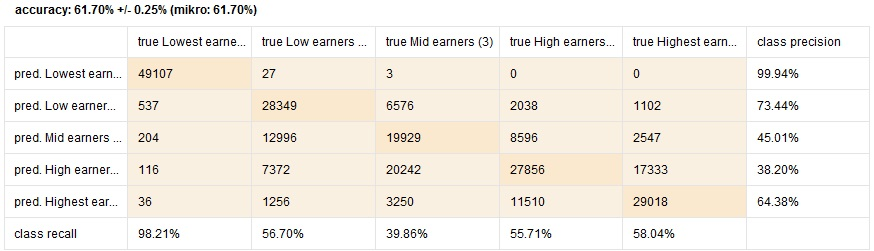
\includegraphics[scale=.55]{pictures/5classErrorTrain} \\
	Error on testing:\\
	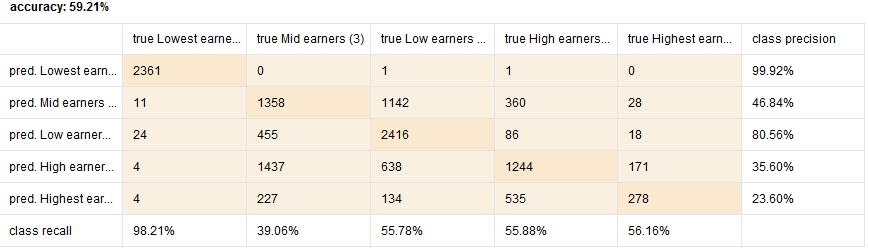
\includegraphics[scale=.55]{pictures/5classErrorTest}
}

\frame{
	\frametitle{Prediction of High Earners}
	\framesubtitle{Decision Tree - information\_gain, maximal depth 6, no pruning}
	\pause
	Two earner classes: high earners and all the others\pause
	\begin{itemize}
		\item same preprocessing as in the 5 classes case \pause
		\item again too many attributes $\rightarrow$ forward selection operator: \pause
		\begin{itemize}
			\item \textbf{iYearsch}, \textbf{iFertil}, \textbf{dWeek89}, \textbf{iClass}, \textbf{dHour89}, \textbf{iTmpabsnt}
			\item \textbf{dIndustry} - specification of industry
			\item \textbf{iRelat1} - relationship to householder
			\item \textbf{dOccup} - occupation
			\item \textbf{iDisabl2} - work limitation status
			\item \textbf{iSept80} - served September 1980 or later
			\item \textbf{iWorklwk} - worked last week \pause
		\end{itemize}
		\item 83.29\% accuracy on training data with 10-fold cross validation \pause
		\item 79.72\% accuracy on test dataset
	\end{itemize}	
}

\frame[plain]{
	Error on training:
	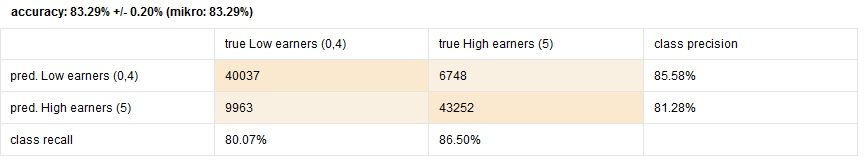
\includegraphics[scale=.6]{pictures/highEarnerErrorTrain} \\
	Error on testing:\\
	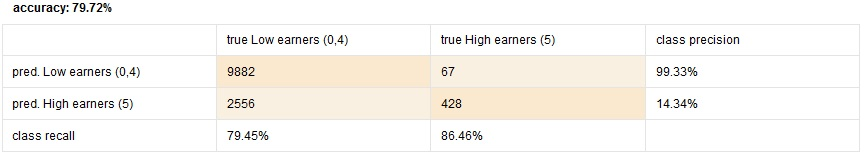
\includegraphics[scale=.6]{pictures/highEarnerErrorTest}
}

\frame{
\centering \huge The End	
}

\end{document}
